
\vspace{1cm}{\bf ECal performance [Sho]}

The ECal preamplifiers shape the APD signal into a CR-RC pulse of rise time $\approx 14$ ns; this is sampled every 4 ns and stored in a pipeline on the FADC readout board.
On receiving a trigger, the FADC searches for rising threshold crossings in the pipeline, and integrates pulses by summing 5 samples before and 30 samples after each threshold crossing.

The noise and pedestal of the readout chain are calibrated by running the

Of 442 crystals/channels, 39 were disabled or disconnected and were not read out by the DAQ. 
13 of these were not read out because of a shortage of FADC readout boards.
The remainder either had no HV bias on the APD, or were disabled in the FADC software due to noise.

In the data, we identified two types of abnormal channels. 
One FADC was not sending trigger signals correctly, resulting in low efficiency. This affected the 13 channels read out by that FADC.
5 channels were diagnosed as noisy because they had a high incidence of hits out of coincidence with the trigger.

A large number of channels were originally misidentified as noisy because they had much higher hit occupancy than neighboring channels.
Gain calibration (described in the next section) shows that these channels have high gain (and thus lower energy threshold) but are otherwise normal.

The abnormal channels were ignored in analysis in order to simplify comparison with Monte Carlo. This leaves 385 useful channels---87\% of the ECal.

We found that one quadrant of the ECal had been miswired in such a way as to flip the horizontal coordinate---the column of crystals nearest the center was connected to the readout channels for the rightmost column, and vice versa.


Describe clustering, thresholds, occupancy, dead/noisy crystals, flip in readout?

Plots: Occupancy map

\begin{figure}[ht]
	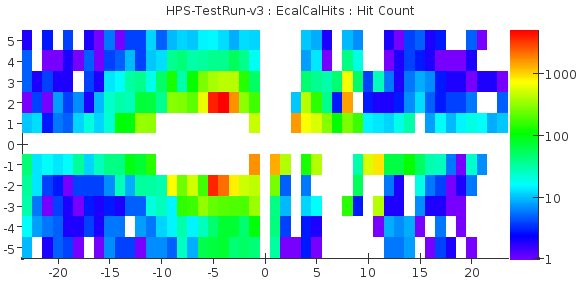
\includegraphics[width=0.5\textwidth]{test2012/ecalperformance/hitrates}
	\caption{\small{}}
	\label{fig:hitrates}
\end{figure}

\vspace{1cm}{\bf ECal Calibration [Sho]}


Description of the gain calibration. Relate to how good it needs to be which should be in the performance section. Discussion of sampling fraction. Relation to what calibration that is needed for the trigger in 2014?

Plots: E/p map before and after calibration, spread in gain, E/p data/MC


\vspace{1cm}{\bf Trigger performance [Sho/Ben]}

%\begin{figure}[ht]
%	\includegraphics[width=\textwidth]{test2012/ecalperformance/trigtimes}
%	\caption{\small{}}
%	\label{fig:trigtimes}
%\end{figure}

As described in Section \ref{sec:tesrun_trigger}, the trigger and DAQ integrate pulses differently to measure hit energy. The trigger integrates using a time-over-threshold window, and the DAQ readout integrates using a constant window (5 samples before and 30 samples after a threshold crossing). 

For every event, the trigger reports as a bitmask the trigger decision (top trigger, bottom trigger, or both) and the time the trigger fires.

We study trigger performance by simulating the trigger for each event and comparing actual To study trigger performance, we first convert from readout hits (constant integration window) to trigger hits (time-over-threshold integration). 
This is done by converting from the readout hit to pulse amplitude, then applying the time-over-threshold algorithm to the simulated ECal pulse shape. 
We then simulate the CTP clustering algorithm and the trigger decision, and compare the trigger decision and trigger time reported by the simulation to what was reported by the real trigger.

To eliminate trigger bias in checking the trigger decision, we use a tag and probe method: to check trigger performance in one half of the ECal, we tag events where there was a trigger in the other half, and exactly one probe cluster in the ECal half under test. 
We then measured trigger efficiency (proportion of tagged events where there was a trigger) as a function of ADC counts and energy of the probe cluster.

These turn-on curves are shown for the top half of the ECal in Figure \ref{fig:turnon}. 
The trigger threshold is seen to be 1280 ADC counts as expected; the threshold is not perfectly sharp in this analysis because of uncertainties in the conversion from constant-window to time-over-threshold integrals, but based on comparisons with Monte Carlo simulation we believe the trigger worked exactly as specified. 
The trigger threshold in terms of cluster energy is very uneven for two reasons: gain variations between different ECal crystals lead to threshold variations, and the nonlinearity of the time-over-threshold integral means that the effective threshold is higher for clusters that span multiple crystals.

\begin{figure}[ht]
	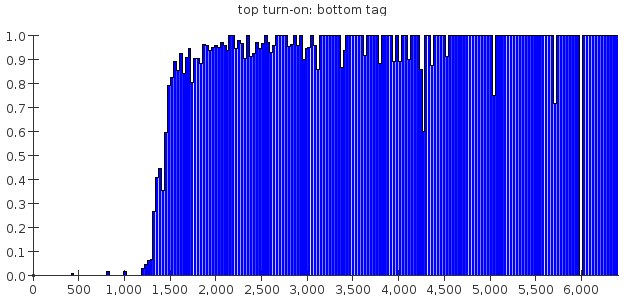
\includegraphics[width=0.4\textwidth]{test2012/ecalperformance/top_turnon_adc}
	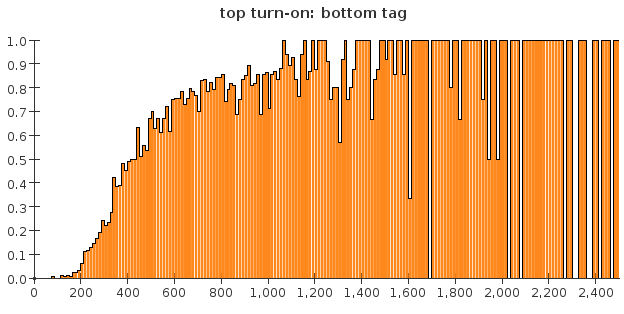
\includegraphics[width=0.4\textwidth]{test2012/ecalperformance/top_turnon_e}
	\caption{\small{Trigger turn-on as a function of probe cluster ADC counts (left) and probe cluster energy in MeV (right). Both plots are for the top half of the ECal; bottom is similar. 
	Energy is not corrected for sampling fraction.}}
	\label{fig:turnon}
\end{figure}

Overall the trigger appears to have functioned exactly as intended. Changes planned for the next run (constant integration window and per-crystal gain calibration constants for the trigger) will solve both of the issues that led to threshold variations in the test run.

What were the rates, lessons learned?

Plots: Compare observed and expected trigger time {\it Sho}, Tag\&probe {\it Sho}, rates vs time {\it Ben/Sho/Pelle}


